\section{Appunti di Tue 21 May 2019 02:48:28 PM CEST}

Potenza
\begin{itemize}
    \item Statica = 0
    \item Dinamica

        $\rightarrow$ Cortocircuito

        $\rightarrow$ Carico
\end{itemize}


\begin{figure}[ht]
    \centering
    
\includegraphics[width=1.8in]{placeholder.jpg}
    \caption{Grafico 1}
\end{figure}

\begin{samepage}
\[
    I_{D} = \frac{\beta}{2}{\left\{\frac{t}{t_R} V_{DD} - V_{T} \right\}}^2
\]

\[
    V_i(t) = \frac{t_1}{t_r} V_{DD} = V_T \rightarrow t_1 = \frac{V_t}{V_{DD}} t_R
\]

\[
    V_i(t_5) = \frac{t_5}{t_R} V_{DD} = \frac{V_{DD}}{2} \rightarrow t_5 = \frac{t_R}{2}
\]

\[
    \tilde{P} = \frac{1}{T}\int_{0}^{T} V_{DD}I_{D}dt =
    \frac{1}{T} 4 \int_{t_1}^{t_5} V_{DD} \frac{\beta}{2} \left( t \frac{V_{DD}}{t_R} - V_T\right) ^2 dt
\]

\[
    =\frac{4}{T} \frac{\beta V_{DD}}{2} \frac{t_R}{3}
    \left[ \left( t \frac{V_{DD}}{t_R} - V_T\right)^3\right]^{\frac{t_R}{2}}_{\frac{V_T}{V_{DD}} t_R }
\]

\framebox{$\tilde{P_{CC}} = \frac{\beta}{2} \frac{t_R}{T} \left( V_DD - 2 V_T\right)^3$}

% Riprende da ?
\end{samepage}

\begin{figure}[H]
    \centering
    \begin{circuitikz}
        \draw(0, 0) node[eground]{}
        to[Tnmos, n=tnm] ++(0, 1.5)
        to[Tpmos, n=tpm] ++(0, 1.5)
        -- ++(0, 0.2)
        node[vcc]{$V_{CC}$};

        \draw(tnm.G) -- (tpm.G);

        \draw (tnm.D -| tnm.G) to[short, -*] ++(-0.5, 0);
        \draw(tnm.D) -- ++(1, 0)
            to[C] ++(0, -1)
            node[eground]{};

    \end{circuitikz}
    \caption{Circuito 1}
\end{figure}

Applicando Kirkoff: $I_{DP} = I_{Dn} + I_C$

Ricostruita la situazione possiamo analizzare la potenza media associata al carico $\tilde{P_i} = \frac{1}{T}\int_0^T I_{DD} V_{DD} dt $

Sempre dalla relazione di prima, siccome $I_C = 0 \Rightarrow I_{DD} = I_{DP}$


P-mos \'e \textbf{saturo} quando \framebox{$ V_u < V_i + V_t $}

Istantaneamente posso avere un bilancio energetico non nullo, ma in un caso periodico somma dell' energia, per il principio di conservazione deve essere nulla

Sommando le tre potenze devo trovare la potenza complessiva, quindi:
\[
    \tilde{P_L} = \tilde{P_n} + \tilde{P_p} + \tilde{P_C}
\]

\[
    \tilde{P} = \frac{1}{T}\int_0^T  V_U I_C dt = \frac{1}{T} \int_0^T V_U C_L \frac{dV_U}{dt} dt =
    \frac{C_L}{T}\int_{V_U(0)=0}^{V_U(T) = 0} \cdots = 0
\]

Ovvio che \'e nullo perche l'energia di un condensatore \'e legata alla carica

\[
    \tilde{P_P} = \frac{1}{T} \int_0^T V_{BDP} I_{DP} dt = \frac{1}{T}\left[ \int_0^{\frac{T}{2}} V_{BD} I_{DP} dt + \int_{frac{T}{2}}^{2T} V_{SD}I_{DD}dt\right]
\]


\[
    \frac{1}{T} \int_0^{\frac{T}{2}} (V_{DD} - V_U) C_L \frac{dV_U}{dt}dt = -\frac{C_L}{T} \int (V_U - V_{DD}) dV_U = \cdots
\]

\[
    =\frac{C_L}{T} \frac{V_{DD}}{2}^2
\]

Calcolando la potenza consumata dal transitorio di Pull Down (N-mos)
Osservando che nel primo semiperiodo l'n-mos \'e spento, La corrente \'e nulla, quindi ci limitiamo ad integrare nel secondo semiperiodo
\[
    \tilde{P} = \frac{1}{T}\int_0^T  V_U I_C dt = \frac{1}{T} \int_{\frac{T}{2}}^T V_U C_L \frac{dV_U}{dt} dt =
\]

Sapendo che $I_{DD} = -C_L\frac{dV_U}{dt}$ Abbiamo che:

\[
    -\frac{C_L}{T} \int_{V_U(T/2) = V_{DD}} ^ {V_U(T) = 0} V_U \frac{dV_U}{dt} dt = \cdots = \framebox{$\frac{C_L}{T} \frac{V_{DD}^2}{2}$}
\]

Quindi: $\quad \tilde{P_L} = \frac{C_L}{T} {V_{DD}^2} $

Si pu\'o notare che la potenza dissipata non dipende dai parametri dei transitori ($\beta$ non compare nell' espressione)

Siccome quello che mi serve \'e caricare il condendatore, devo spendere un energia doppia rispetto a quella che $\cdots$

Se cambia $\beta$ cambia solo il tempo in cui si carica/scarica il condensatore, $\beta$ non influisce sull'energia

$ \frac{1}{T} = f  \Rightarrow  f C_L {V_{DD}}^2$

Questa che \'e una potenza dinamica, aumenta con la frequenza $\rightarrow$ devo caricare e scaricare il condensatore pi\'u volte

In $P_{CC}$ Compare il rapporto  $\frac{t_R}{T}$, supponendo di essere capaci di far andare pi\'u veloce il circuito, il rapporto tende a rimanere costante $\rightarrow$ Ridurre il periodo aumenta la potenza associata a carica-scarica, ma ha un effetto limitato sulla potenza di cortocircuito

La frequenza sicuramente cresce perche siamo sicuri di riuscire a fare dispositivi pi\'u veloci, ma fare dispositivi piu piccoli, lo scopo della riduzione delle geometrie non \'e fare lo stesso circuito pi\'u piccolo, ma per poter mettere pi\'u ``roba'' all'interno dello stesso chip.

Viene sfruttata la possibilit\'a di mettere pi\'u componenti nello stesso spazio, la frequenza di clock dipende anche dall'architettura e da come \'e fatto il circuito

\begin{figure}[ht]
    \centering
    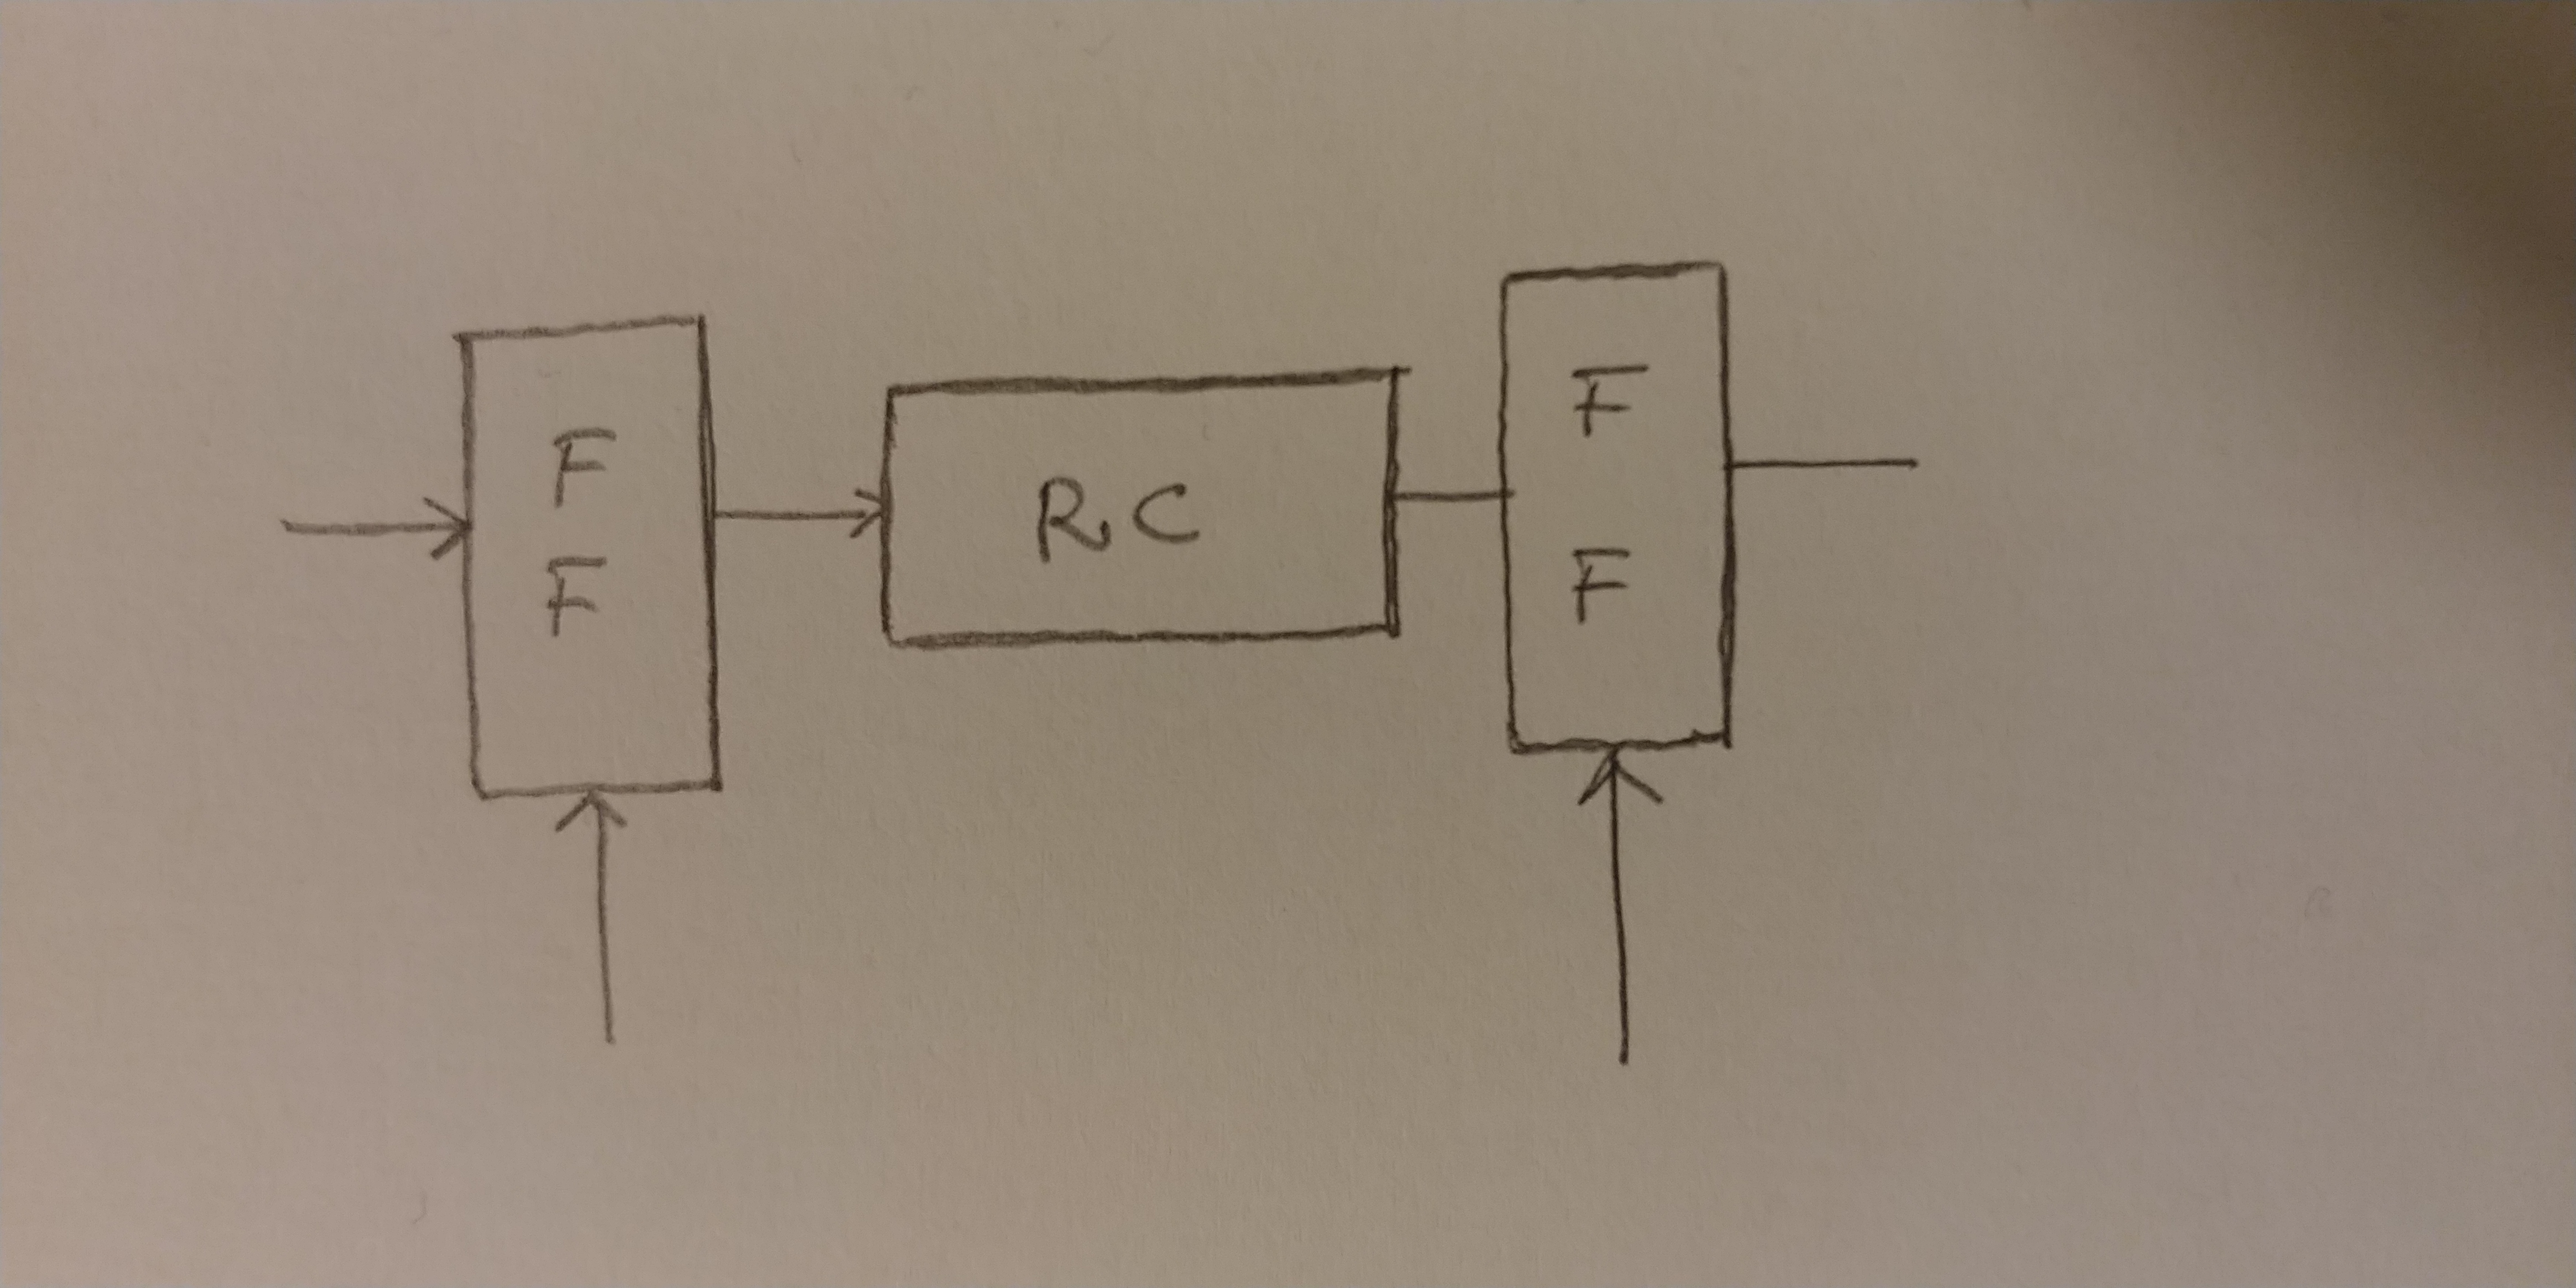
\includegraphics[width=3in]{img/elettronica/esempio_clock.jpg}
    \caption{Esempio di clock}
\end{figure}

Rete sincrona \'e piu robusta e piu sicura al problema delle Alee, il periodo di clock deve garantire che tutta la rete combinatoria, abbia il tempo di completare il suo lavoro.

La possibilit\'a di integrare circuiti pi\'u complessi viene sfruttata per implementare architetture con maggiori prestazioni, es. Circuiti in Parallelo

Siccome abbiamo scoperto che la frequenza di clock impatta direttamente sulla frequenza associata al carico, e tende ad aumentare con la riduzione delle dimensioni, comporta al fatto che, se tutto il resto rimanesse costante, tutto va pi\'u veloce e consuma di pi\'u perche va piu veloce: Utilizzo architetture con maggiore prestazione a cui \'e associato un maggiore consumo

Circuiti c-mos caratterizzato da un basso consumo di potenza statico, ma un alto consumo dinamico

Differenza fondamentale con la logica RTL era che quella consumava sia che lavorasse, sia che non lavorasse

Logica di tipo \textbf{ratioless}: Le dimensioni del transistore non impattano sulla funzionalit\'a

